\documentclass[11pt]{article}
\usepackage{tikz}
%\usepackage{xfrac}
%\usepackage{hyperref}
%\usepackage[export]{adjustbox}
\def\checkmark{\tikz\fill[scale=0.4](0,.35) -- (.25,0) -- (1,.7) -- (.25,.15) -- cycle;} 
\usepackage{proj} 	% pull in style header
\usepackage{array}
\usepackage{sectsty}
\usepackage{soul}
\usepackage{float}
\usepackage{multirow} 
\usepackage{gensymb}
\restylefloat{table}

\lhead{ECE544: Embedded Systems on FPGAs}


%----------------------------------------------------------------------------------------
%	TITLE SECTION
%----------------------------------------------------------------------------------------


\newcommand{\horrule}[1]{\rule{\linewidth}{#1}} % Create horizontal rule command with 1 argument of height

\title{	
\normalfont \normalsize 
\textsc{\LARGE Portland State University}\\[1.5cm] % Name of your university/college
\textsc{\Large Embedded Systems on FPGAs}\\[0.5cm] % Major heading such as course name
\textsc{\large ECE544}\\[0.5cm] % Minor heading such as course title
%\textsc{Portland State University} \\ [25pt] % Your university, school and/or department name(s)
\horrule{1.2pt} \\[0.4cm] % Thin top horizontal rule
\huge Autonomous Robot Car \\ % The assignment title
\horrule{1.2pt} \\[0.5cm] % Thick bottom horizontal rule
}

%----------------------------------------------------------------------------------------
%	AUTHOR SECTION
%----------------------------------------------------------------------------------------


\begin{document}\raggedright
\author{Erik Rhodes \and Caren Zgheib} % Your name
\maketitle % Print the title
\thispagestyle{empty}
\cfoot{\textit{Page \thepage { of} \pageref{LastPage}}}
\lhead{ECE544}
\chead{Final Project}
\rhead{Erik Rhodes \& Caren Zgheib}


\begin{figure}[h]\centering
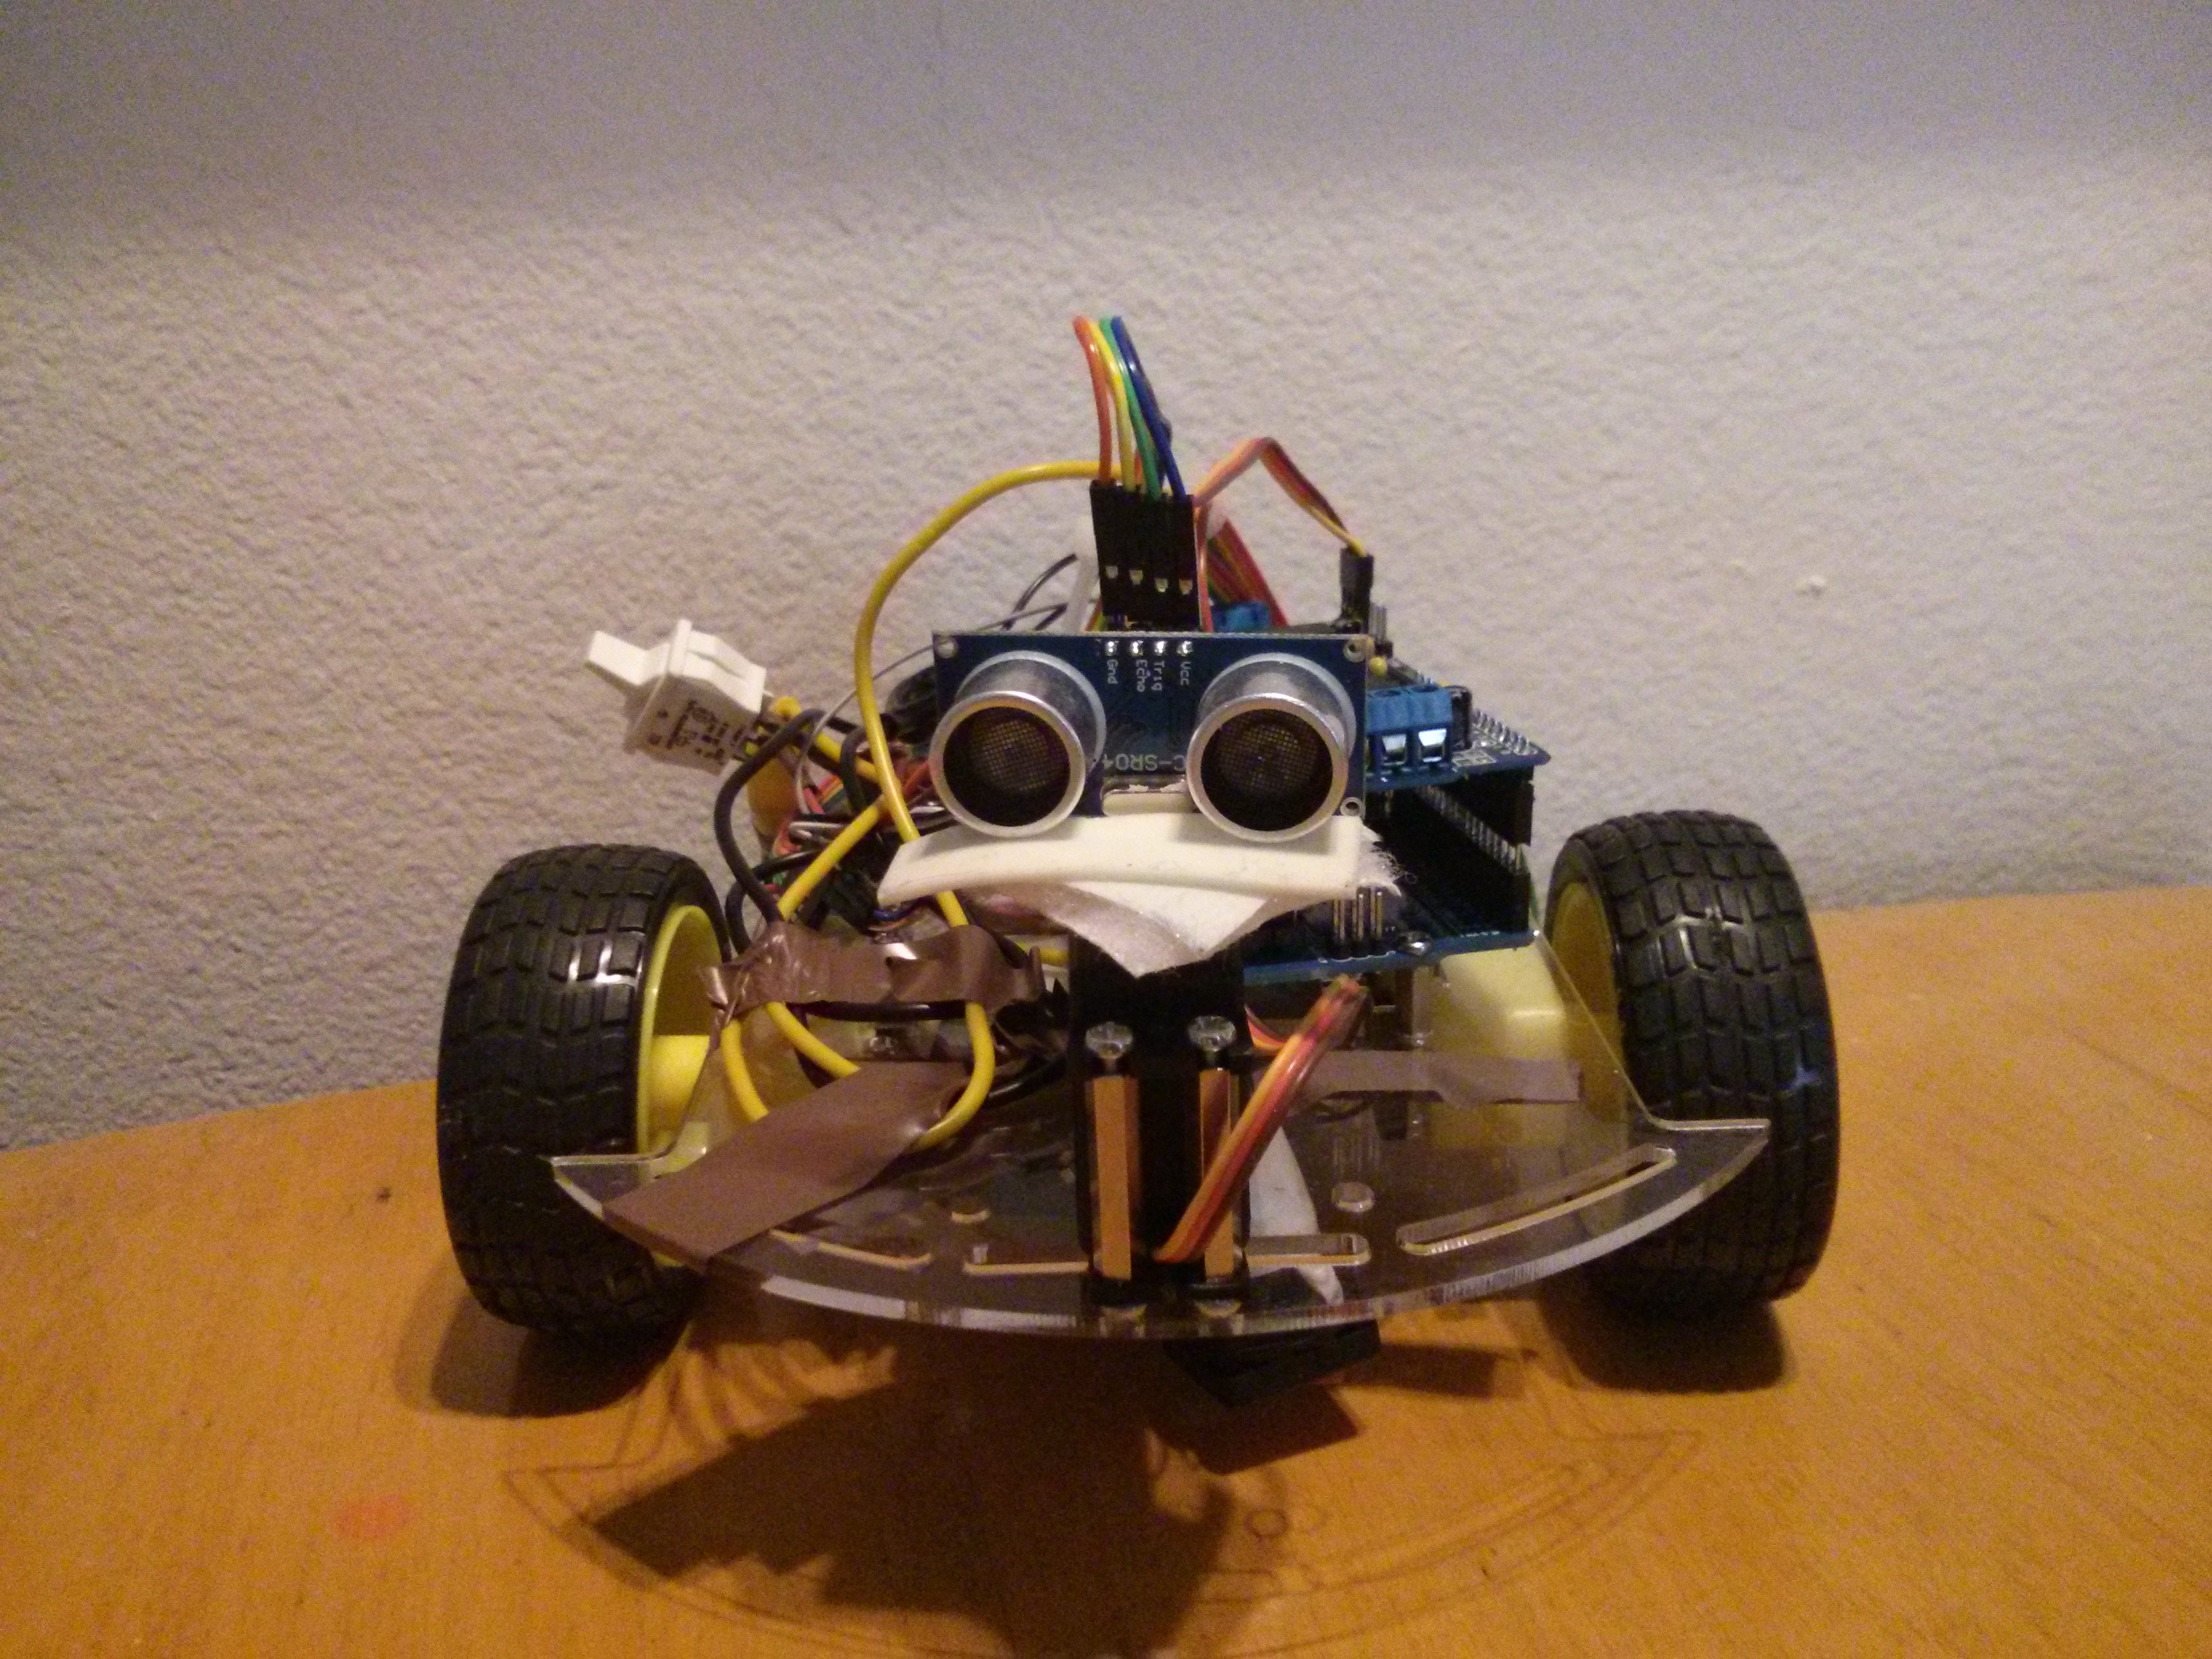
\includegraphics[height=0.65\textwidth]{images/bot_front.jpg}
	%\caption{Gameplay Block Diagram}
		\label{bot_front}
	\end{figure}
	
\tableofcontents
\newpage

% -------------------------PROJECT DELIVERABLES -----------------------------------

% ----------------------------------------------------------------------------------

\section{Introduction} 
We created an autonomous robot car (Sammy) that can successfully navigate its way through a given area without hitting any objects (usually).  It uses the popular \textbf{Arduino} platform and libraries along with a ultrasonic sensor for object detection.  

	\begin{figure}[h]\centering
	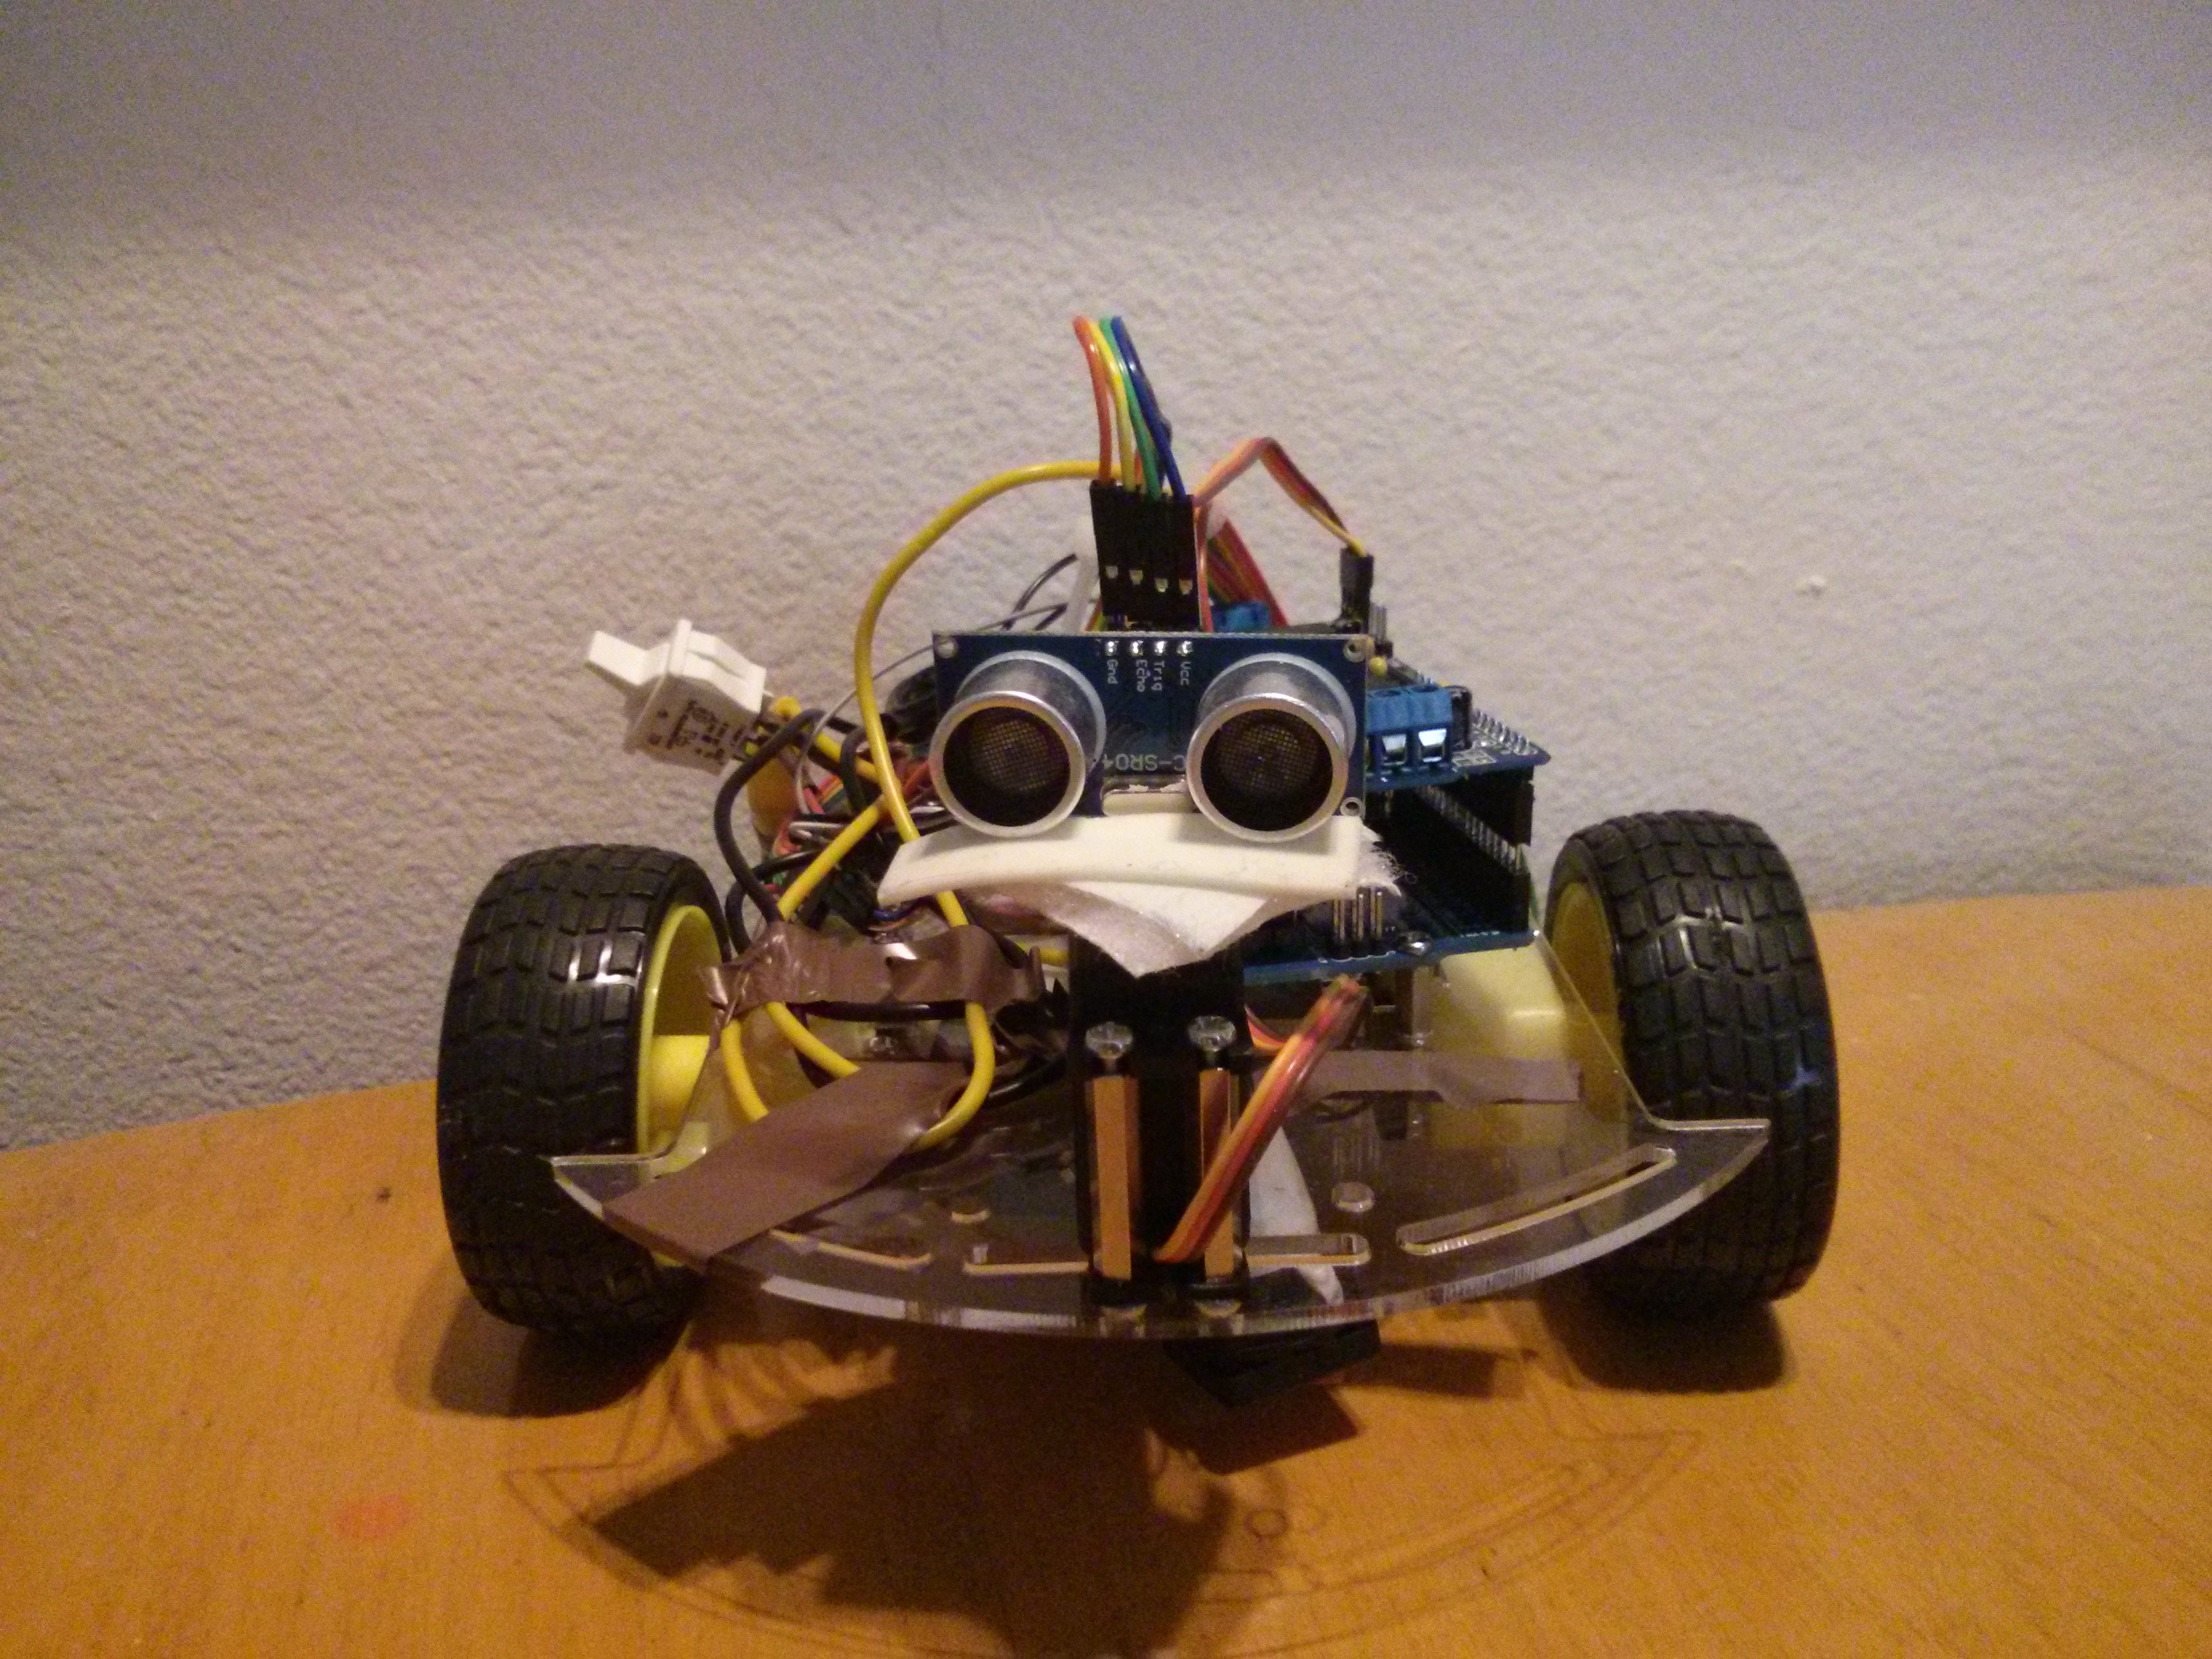
\includegraphics[height=0.7\textwidth]{images/bot_front.jpg}
	\caption{Block Diagram of Control System}
		\label{diagram}
	\end{figure}


%TODO 
% Software algorithm code
% Make flowchart look good
% Label picture of car


%Features

%Components (hardware)
%-pictures?
%-diagram?
%Algorithm (software)
%-flowchart
%-some code
%-scans to left and right when going forward...
%-scans ...

%references
%-oddwires
%-arduino}



\section{Hardware Components}
%TODO Reference
Show diagram of components on the picture...



\section{Robot Control}

\subsection{Functions}
Motor
%Motor
%-Drive Forward
%-Drive Backward
%-Turn left/right
%-Veer left/right
%-U turn
%-Victory Dance

	\begin {table}[h]
	\begin {center} 
	\vspace{15pt}
	
	\begin{tabular}{||c|c|c||}\hline	
		\textbf{Component}	&	\textbf{Function}	&	\textbf{Details}		\\\hline
		\multirow{5}{*}{Motor}
						&	Drive Forward		&	Both wheels moving forward at predefined speed 		\\
						&	Drive Backward		&	Both wheels moving forward at predefined speed 		\\
						&	Turn Left/Right		&	Both wheels spin for ``in-place'' turn of 90\degree	 	\\
						&	Veer Left/Right		&	Only outside wheel turns and vehicle does not stop\\
						&	U-Turn				&	Backs up then turns 180\degree		\\
						&	Victory Dance		&	After certain time, bot does various spins	\\\hline
		\multirow{2}{*}{Sonar + Servo}
						&	Look Forward		&	Scans a 40\degree range in front while moving forward \\
					&	Look Left/Right		&	Scans 90\degree left/right to determine next turn \\\hline

%TODO Mention intervals of 10 degrees and how they are averaged

		
	\end{tabular}
		\caption {Robot Functions} \label{functions}
	\end{center}
	\end{table} 	

Sonar and servo
%scan partial left and right when driving forward, get average
%scan fully left and right, get average
%


\vspace{12pt}

 \begin{lstlisting}[caption=Control Loop, label=loop]		
void loop() {
    if (scanClear())  // If clear to go forward
    {
      drive_forward();
    }
    else              // if path is blocked
    {
      freewheel();    // stop
      lookLeft();
      int distanceLeft = getAverageDistance();

      lookRight();
      int distanceRight = getAverageDistance();
      
      // re-center the ultrasonic
      servo_position(CENTER);

      // go the least obstructed way
      if (distanceLeft > distanceRight && distanceLeft > dangerThreshold)       
      {
        drive_backward();
        delay(400);
        rotate_left();
      }
      else if (distanceRight > distanceLeft && distanceRight > dangerThreshold) 
      {
        drive_backward();
        delay(400);
        rotate_right();
      }
      else 		// equally blocked or less than danger threshold left or right
      {
        freewheel();
        delay(20);
        drive_backward();
        delay(500);
        u_turn();
      }   
    } 
  }  
}
  \end{lstlisting}

\subsubsection{PID}
The more prevalent method, PID, involves making multiple calculations to predict the accurately control the behavior of the output.  The proportional (P) method involves using the previous error margin to calculate the next appropriate one.  The integral (I) method calculates how the system behaves over time, and the derivative (D) calculates how fast the output is changing at that point in time.  Our implementation is seen in listing \ref{PID}. \\
Using a specific arrangement of these parameters will yield a large increase in accuracy, so tuning the application is desirable.  When tuning, we first attempted to follow the \emph{Ziegler-Nichols} method.  After understanding how each method changes the output, we modified the parameters as we saw fit to acquire the most accurate configuration for our control system. 

\vspace{12pt}

 \begin{lstlisting}[caption=PID Algorithm, label=PID]		
     for (smpl_idx = 1; smpl_idx < NUM_FRQ_SAMPLES; smpl_idx++)
     {
         delay_msecs(100);
 
         // get count from light sensor and convert to voltage 
         sample[smpl_idx] = LIGHTSENSOR_Capture(LIGHTSENSOR_BASEADDR, slope, offset, is_scaled, freq_min_cnt);
         volt_out = (-3.3 / 4095.0) * (sample[smpl_idx]) + 3.3;

         // calculate derivative;
         error = setpoint - volt_out;
         deriv = error - prev_error;
 
         // calculate integral
         if (error < setpoint/10) integral += error;
         else integral = 0; 
 
         // Control offset is gotten from characterization
         volt_out = offset + (error * prop_gain) + (deriv * deriv_gain) + (integral * integral_gain);
         duty_out = (volt_out)* (MAX_DUTY+1)/VOLT_MAX;
 
         // establish bounds
         if (duty_out < 1) duty_out = 1;
         if (duty_out > 99)duty_out = 99;
 
         // activate PWM
         Status = PWM_SetParams(&PWMTimerInst, pwm_freq, duty_out);
         if (Status == XST_SUCCESS)	 PWM_Start(&PWMTimerInst);
     } 
  \end{lstlisting}
  
  


\subsection{Peripheral Interface}
The \textbf{TSL237} light-to-frequency converter outputs a period that directly corresponds to the intensity of the light emitted from the LED.  The PWM detection module receives this information and converts it to a ``count'', which is then scaled to fit within the parameters (between 0 and 4095) needed for our control calculations.  These functions are handled in the light sensor driver.  The driver initially converted the scaled counts to a voltage, but we later decided to move that functionality to the program application.
The peripheral has the user-visible registers described in table \ref{registers}.

	\begin {table}[H]
	\begin {center} 
	\vspace{15pt}
	
	\begin{tabular}{||c|c|c|c||}\hline
		\textbf{Register}	&	\textbf{Number}	&	\textbf{Format} 	& 	\textbf{Description}		\\\hline
		Control				&	slv\_reg0		&	{RESERVED[30:0], EN} &  Enable of the peripheral 		\\\hline
		Status				&	slv\_reg1		&	{RESERVED[30:0], EN} & Current settings of the peripheral		\\\hline
		HighTime			&	slv\_reg2		&    HighTime[31:0] 	&	Detected high time count  			\\\hline
		Period				&	slv\_reg3		&  	Period[31:0] 		&	Detected period count 			\\\hline
		SpareReg1			&	slv\_reg4		&	RESERVED[31:0] 		& 	No specific purpose 			\\\hline
		SpareReg2			&	slv\_reg5		&	RESERVED[31:0] 		& 	No specific purpose 			\\\hline
	\end{tabular}
		\caption {Lightsensor peripheral registers} \label{registers}
	\end{center}
	\end{table} 
	

\subsection{Frequency detection}
%TODO Include info about how the detection worked
The measurements output by the light sensor were received by a hardware module that interpreted the data.  This Verilog program closely resembles the PWM detection module done in project 1.  It increments the count on each clock edge, depending on whether the input is high or low.  Once a full period is detected, the high count and period are sent to registers which are able to be read by the light sensor driver.  

\subsection{User Controls} 
The program starts by characterizing the system.  This allows the initial scaling to be performed, which varies by the amount of light detected by the light sensor. After this is done, the default control parameter values are displayed and the user is given a chance to change them.  The type of test and starting input voltage can also be selected.  Once these have been configured, the user starts the test with the rotary button.  When it has finished, long pressing on the rotary button sends the data to the computer connected serially via the UART port.  If the user wants to change the test, they can modify the switch values and update the LCD by pressing on the rotary button.  While the user interface remained close to the recommended specifications, it also included a few features that made it amazingly incredible. The control assignments are seen in table \ref{controls}.
 
 
	\begin {table}[h!]
	\begin {center} 
	\vspace{15pt}
	
	\begin{tabular}{||c|c|c||}\hline	
		\textbf{Name}	&	\textbf{Value}	&	\textbf{Function}		\\\hline
		Switch[1:0]		&	00		&	Bang Bang 		\\\hline
		Switch[1:0]		&	01		&	PID 		\\\hline
		Switch[1:0]		&	10		&	Unused	 	\\\hline
		Switch[1:0]		&	11		&	Characterization 		\\\hline
		Switch[2]		&	0		&	Vin Low		\\\hline
		Switch[2]		&	1		&	Vin High	\\\hline
		Pushbutton		&	North	&	Move Cursor		\\\hline
		Pushbutton		&	East	&	Increase Value		\\\hline
		Pushbutton		&	West	&	Decrease Value		\\\hline
		LCD Display 	&	Row 1	&	PID Values	\\\hline
		LCD Display 	&	Row 2	&	Setpoint and Offset	\\\hline
		Rotary Encoder	& Clockwise	& 	Increase Setpoint		\\\hline
		Rotary Encoder	& Counter-Clockwise	& 	Decrease Setpoint		\\\hline
		Rotary Encoder	& Press Button		& 	Next section \\\hline
		Rotary Encoder	& Long Press Button	& 	Initiate test \\\hline
		
	\end{tabular}
		\caption {Nexys3 Controls} \label{controls}
	\end{center}
	\end{table} 		
  


\section{Conclusion}
\texttt{Servo and Protecto} was quite fun for us to build and was certainly the biggest ``crowd pleaser'' out of all the projects we've made.  The assembly perhaps took the least amount of time, although we did face problems with a few of the parts not being built correctly (mainly the battery holder and motor plate mount).  Fixing the power problems was the most frustrating part of the project, but once we finished everything, the final product was quite rewarding.  We both spent equal times on all the different aspects of this project.  Listed below are some of the challenges we faced.
	
	\subsection{Challenges}
		
		\begin{itemize}				
		\item \textbf{Power Issues}: After the initial assembly, we were not able to properly move the servo and control the motors.  Our initial thought was inadequate power, but the correspondent we communicated with ensured us that it could run perfectly fine on 6V of AA batteries.  Even after upping the voltage we saw problems, which were due to the power demands of our servo.  After increasing the power to 9V of AA batteries the problem diminished.
		\item \textbf{Motor control}: The motors we received are not precise enough to deliver equal power on both sides.  This caused inevitable veering of the robot.  We were able to use our own veering function to correct a lot of this, but were not able to control the bot perfectly.
		\item \textbf{CMUcam}: We were able to calibrate and test the CMUcam, which was intended for color detection.  However, communicating the frames from the camera to the Arduino proved difficult.  Even the example code would not work on our device. We were not able to solve the communication error before the project was due.
		\item \textbf{Erroneous Sonar Readings}: Occasionally the ultrasonic sensor picked up erroneous values that would usually be below 10cm (possibly due to ghost echoes).  This cause the robot to stop immediately.  We adjusted this by filtering out the first ping that it received below 10cm.
		\end{itemize}

\subsection{Future Additions}
The Arduino platform and components in this project provide a large amount of functionality.  Because of this, the amount of improvements is virtually limitless.  Our goals in the future could involve adding:
		\begin{itemize}				
		\item \textbf{Battery Pack}: Buying a powerful, rechargeable battery pack would save money, improve performance and decrease hassle.
		\item \textbf{External Apparatus}: We initially wanted to attach a simple device that could be triggered based on certain events.  While launching or shooting an object would have been interesting, in most cases this would require PID algorithms, which would involve sufficiently more work and tuning.
		\item \textbf{Color Detection}: One of our original ideas (and part of the reason for the name \textbf{Servo and Protecto}) was to use color detection to differentiate between ``friends'' and ``enemies''.  There would be certain objects that the robot would purposely avoid, and others that it would just run over.
		\item \textbf{Infrared}: Infrared sensors can be used to detect edges, and they could also be used as an external controller/remote.
		\item \textbf{Object Following}: The sonar and/or color detector could be used to follow an object instead of avoid them.  This would be useful when if we attached a physical arm or apparatus of some sort.
		\end{itemize}

\section{References}
Include oddwires stuff?
\end{document}